\section{Localization system}\label{sec:localization-system}

This section details the ROS implementation of the proposed 3/6 DoF \gls{drl}\footnote{\url{https://github.com/carlosmccosta/dynamic_robot_localization}}. It starts with an overview of the main processing stages and then details the control flow and algorithms within the localization pipeline.

\subsection{Overview}

The self-localization system was implemented as a \gls{ros} package and extensible uses the \gls{pcl} \cite{Rusu2011} for its processing pipeline. It provides 3/6 \gls{dof} localization by publishing \emph{geometry\_msgs::PoseStamped} and \emph{geometry\_msgs::TransformStamped} messages along with a detailed analysis of the pose estimation and registered point cloud (split into inliers and outliers). Moreover, it also gives detailed analysis of the computation runtime of each of its modules in order to pinpoint which algorithms are using more computation resources (which is very useful information when configuring or upgrading the system).

The \gls{ros} implementation can receive sensor data through \emph{sensor\_msgs::PointCloud2} messages and as a result it can directly use data from RGB-D and \gls{tof} cameras. To use \glspl{lidar} it provides an assembler that can produce point clouds by merging measurements from several sensor scans using spherical linear interpolation. As such, if the \gls{lidar} sensors are mounted on tilting platforms, they can emulate a 3D sensor and retrieve a very detailed view of the environment.

The self-localization system has a modular software architecture and was implemented as several C++ templated shared libraries that can be easily used for other applications besides robot self-localization. As can be seen in \cref{fig:localization-system_localization-system-brief-overview,fig:localization-system_localization-system-overview}, it is an extensible and flexible system able to fit the needs of a wide range of mobile platforms. It can be configured as a tracking system, with or without pose recovery and can also have initial pose estimation using feature detection and matching. Moreover, it can dynamically create and update the map if necessary.

It supports two configurable processing pipelines in order to allow fast deployment of robots in large environments. One to process new reference maps and another to localize a mobile robot platform using live point clouds. This enables the loading of either processed or unprocessed referenced point clouds and allows a navigation supervisor to dynamically provide the relevant map sections based on the robot position (in order to reduce the computation resources needed by lowering the number of kd-tree levels of the reference point cloud).

\begin{figure}[h]
	\centering
	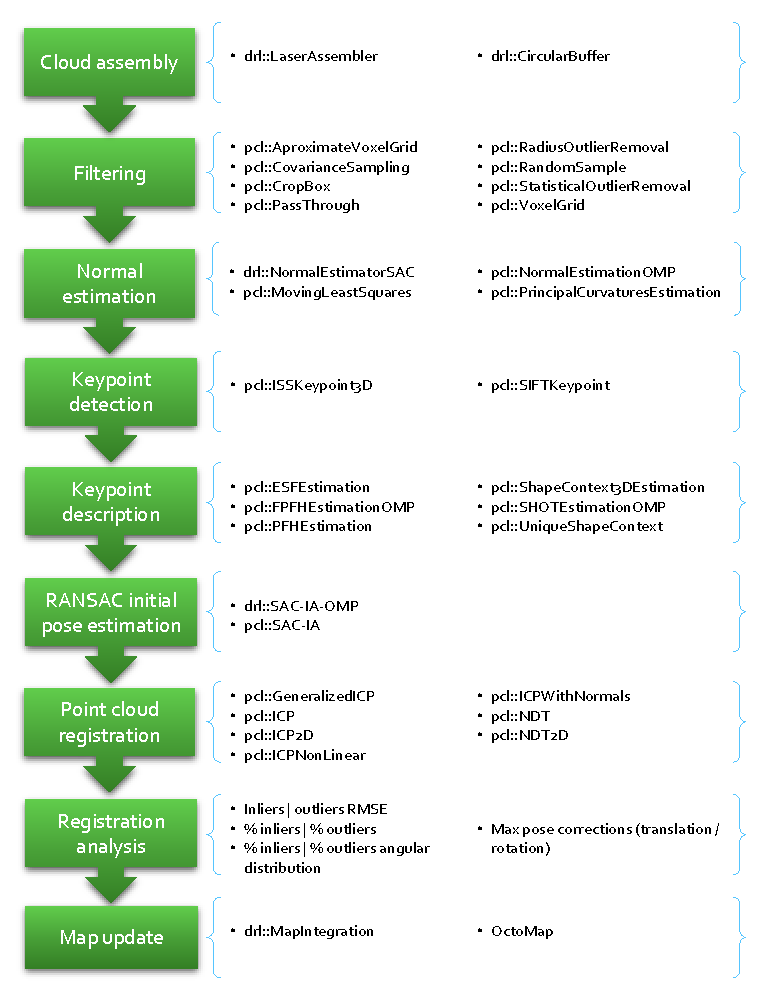
\includegraphics[trim={0.2cm 0.2cm 0.2cm 0.2cm}, clip, width=0.49\textwidth]{localization-system/localization-system-modules}
	\caption{DRL system modules overview}
	\label{fig:localization-system_localization-system-brief-overview}
\end{figure}

\begin{figure}[h]
	\centering
	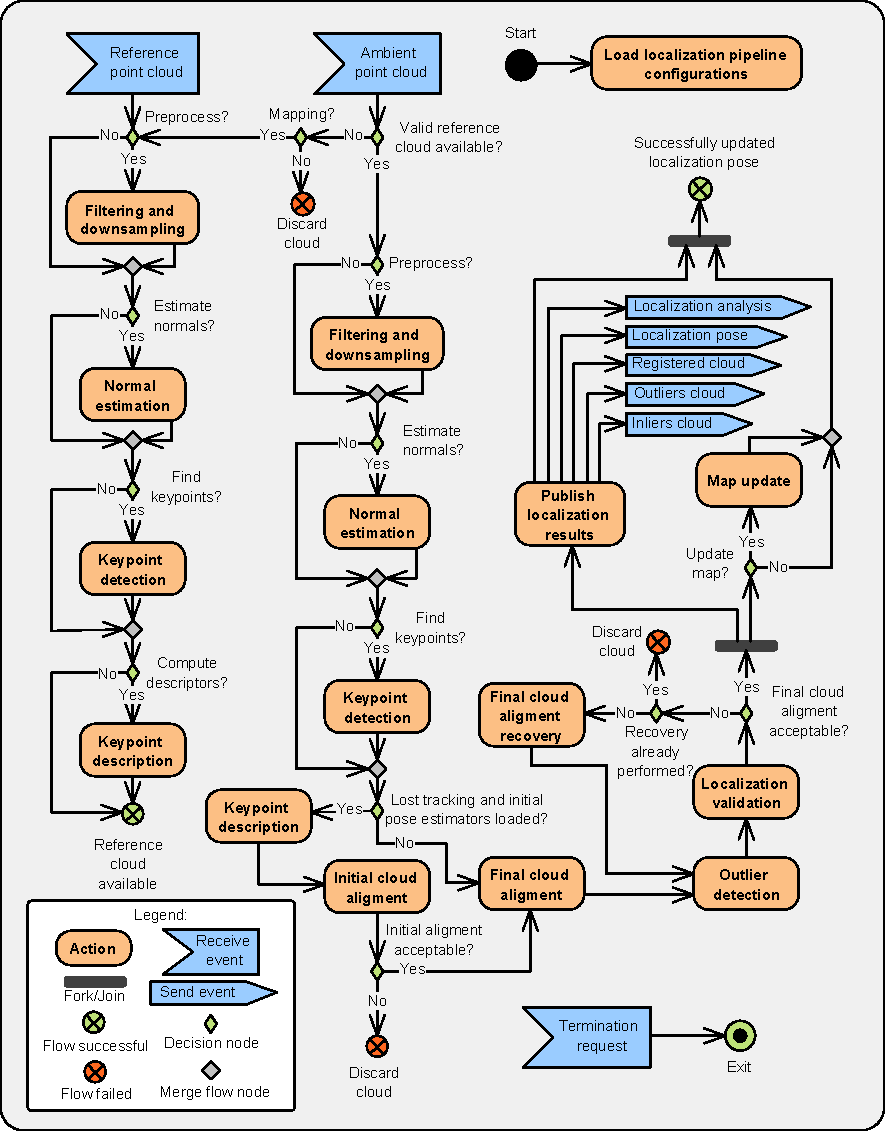
\includegraphics[width=0.49\textwidth]{localization-system/localization-system-overview}
	\caption{DRL system detailed processing pipeline}
	\label{fig:localization-system_localization-system-overview}
\end{figure}


\subsection{Pipeline configuration}

The self-localization system was designed to allow fast reconfiguration\footnote{\url{https://github.com/carlosmccosta/dynamic_robot_localization/blob/hydro-devel/yaml/schema/drl_configs.yaml}} and parameterization through the use of yaml files and the \gls{ros} parameter server. This gives the possibility to quickly tune the localization system to the specific needs of a given mobile platform moving in a particular environment, in order to use the least amount of computational resources possible and without requiring any reprogramming or source code modification. Nevertheless, the system can use a generic configuration if hardware resources are not a concern.

In a typical configuration (following the \emph{Yes} paths of the activity diagram in \Cref{fig:localization-system_localization-system-overview}), the first time the localization system is used, it receives a raw reference point cloud that is preprocessed and saved to long term memory along with its associated keypoints and keypoint descriptors. This allows a much faster startup the next time the localization system is initialized. After having a reference point cloud, the localization system will estimate the robot pose periodically by analyzing the live point cloud sensor data. This data can be preprocessed with several filters and can be associated with computed surface normals. The robot pose estimation is performed by applying a matrix transformation correction to the current robot pose and is based on the registration of the live point cloud with the know map. This registration can use a tracking algorithm configuration tuned for efficiency and a second configuration for tracking recovery purposes. These tracking algorithms require a initial pose estimation, and as such, if one isn't available, a third configuration can be employed to estimate the global position of the robot using geometric features of the environment. The switch between these configuration is based on the analysis of the registered cloud metrics, such as outlier percentage, inliers root mean square error, inliers angular distribution and the registration corrections performed on the live point cloud. After successfully performing the robot pose estimation, the map can be updated by either integrating the full registered point cloud, its inliers or its outliers. Finally, like most \gls{ros} nodes, the localization system will stop its execution when it receives a termination signal request.

The next subsections explain in detail the architecture and algorithms used in each of the processing modules present in \cref{fig:localization-system_localization-system-brief-overview,fig:localization-system_localization-system-overview}.


\subsubsection{Reference map}

The reference point cloud can be loaded from a \gls{cad} file, point cloud file or dynamically arrive trough a \gls{ros} topic as either a 3 \gls{dof} \emph{nav\_msgs::OccupancyGrid} or 6 \gls{dof} \emph{sensor\_msgs::PointCloud2}. This allows a localization supervisor to give only sections of a global map in order to use the least amount of memory and processing time (very large maps have deeper search structures, such as kd-trees, and should be avoided in order keep the number of tree levels within reasonable values).


\subsubsection{Point cloud assembly}

The self-localization system can use any sensor that provides point clouds, namely RGB-D / \gls{tof} cameras, \glspl{lidar} and stereo vision systems. Each of these types of sensors have very different operation rates and measurements accuracy. As such, the localization system allows the assembly of several live scans using a circular buffer in order to reduce the impact of sensor noise.

For \glspl{lidar}, the system provides a \emph{sensor\_msgs::LaserScan} assembler\footnote{\url{https://github.com/carlosmccosta/laserscan_to_pointcloud}} that converts laser measurements in polar coordinates into Cartesian coordinates and projects the points using spherical linear interpolation (in order to account for laser scan deformation that occurs when the robot is moving and rotating). It can merge scans from several lasers sensors and it will publish the final point cloud after assembling a given number of scans or periodically after a specified duration. These assembly configurations can be changed at runtime based on the robot velocity (for example, when the robot moves slower, more laser scans are assembled for each published point cloud) or through the use of the \gls{ros} dynamic reconfigure \gls{api}, which allows a navigation supervisor to control the rate at which the localization system operates.


\begin{figure}[H]
	\centering
	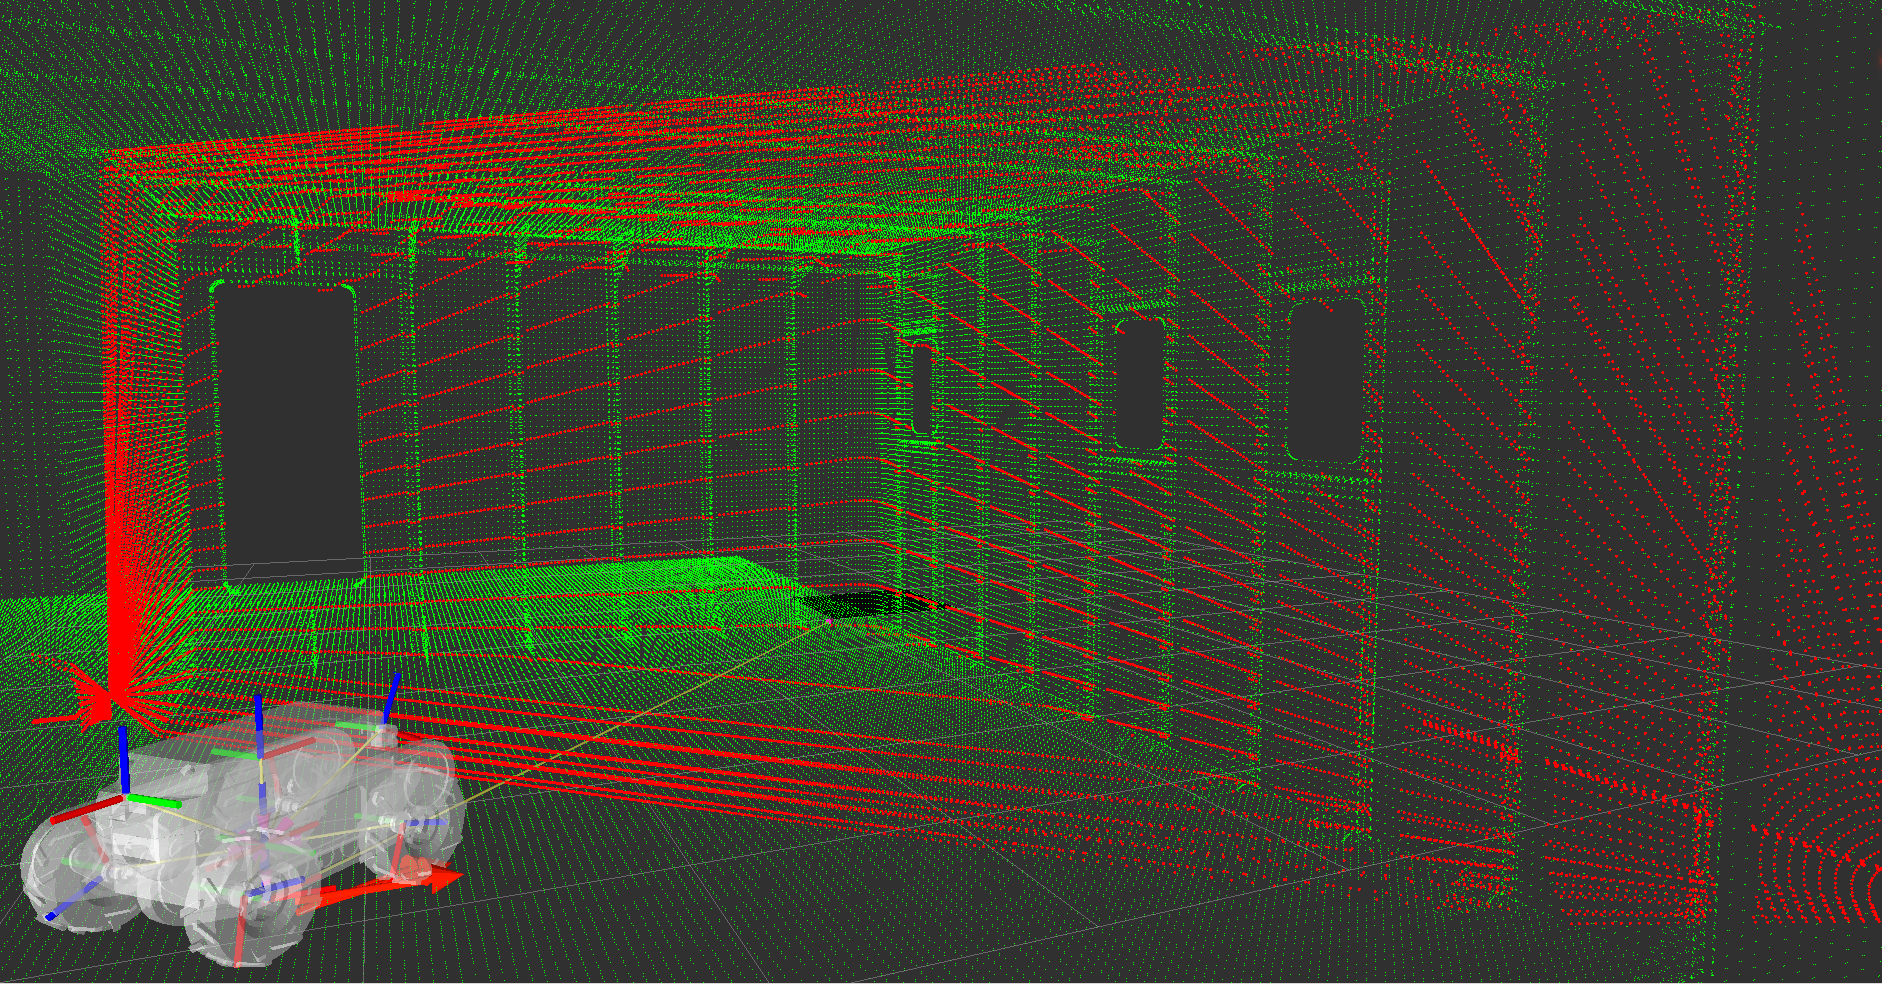
\includegraphics[width=0.48\textwidth]{localization-system/laser-assembly}
	\caption{Laser scans assembled with tilting platform (red points)}
	\label{fig:localization-system_section_laser_assembly}
\end{figure}


\subsubsection{Filtering and down sampling}

The time it takes to perform cloud registration increases considerably when the amount of points in the live point cloud and in the reference map becomes larger. As such, adjusting the level of detail of the point clouds by using voxel grids gives some control over the desired localization accuracy and the computational resources that will be required. This stage is also useful to mitigate the measurement errors of the depth sensors, since the centroid of a voxel that contains points from several scans will be closer to the real surface (if the voxels have dimensions slightly larger than the expected measurement errors).

The localization system allows the application of several preprocessing algorithms (algorithm type / configuration and execution order customizable). The next sections detail some of the methods that can be used to filter and downsample point clouds.


\paragraph{Voxel grid sampling}

A voxel grid is a uniform space partition technique that can be used to cluster points according to their Euclidean coordinates. It is a very effective method to control the level of detail of a point cloud because it gives the ability to specify the maximum number of points that a region of space should have.

The point cloud downsampling is achieved by replacing each voxel cluster with a single point. The selection of this point can be very fast if the voxel center is used (pcl::ApproximateVoxelGrid), but computing the centroid of the cluster (pcl::VoxelGrid) yields better results because it represents the underlying surface with more accuracy and it attenuates errors in the sensors measurements.


\paragraph{Random sampling}

Random sampling \cite{Vitter1984} is a fast downsampling method that randomly selects points from the input cloud until the specified number of samples is reached (pcl::RandomSample). This has the advantage of using real measures instead of downsampled approximations, but also means it is more sensible to sensor measurements noise. However, for outdoor environments or very complex scenes, using the real measurements can be preferable than using cluster centroids because the voxels may not have the necessary resolution or may have a prohibitive computational cost.


\paragraph{Covariance sampling}

Covariance sampling \cite{Gelfand} is a subsampling method that aims to create a stable downsampled point cloud to be registered with \gls{icp} algorithms. It incrementally builds the downsampled point cloud while trying to keep the 6 eigenvalues of the filtered point cloud covariance matrix as close to each other as possible (pcl::CovarianceSampling).

The resultant point cloud has the desired number of points and is stable enough to be matched with \gls{icp} point to plane algorithms.


\subsubsection{Outlier removal}

Some depth sensors can perform measurements with high accuracy, but they have some limitations that can lead to the creation of outliers \cite{Sotoodeh2006}.

One of those limitations can produce shadow points around objects boundaries. This is due to the fact that a portion of the laser beam may hit the object boundary and other part may hit other areas in the object background. And given that most laser range finders use a weighted sum of several beams, this can yield measurements that are not associated with any real object (outliers). Another issue is related to the angle in which the depth sensor sees the objects areas. If the incidence angle is very low, then it may be difficult to compute its distance and detect if the beam had ambient reflections. This can significant increase the measurements noise or even lead to the creation of outliers. Other common problem is associated with the material properties of the surfaces. For example, objects with very high or very low reflectance, such as metals or glass, can increase the measurements noise. Moreover depending on the combination of surface geometry, material and incidence angle, some objects may even be undetectable by depth sensors.

Given the negative effect that outliers have in surface normal computation and registration algorithms, they should be removed in a preprocessing stage. There are several approaches to perform outlier detection and removal \cite{YangZhang2010}, ranging from simple distance thresholds to more robust statistical analysis. The next sections present some of the methods that can be useful in a localization system.


\paragraph{Distance filter}

Given that depth sensors have a minimum and maximum recommended distance for their measurements, it is wise to remove points that are close or beyond these limits. Moreover, it may be useful to remove points that are too close to the sensor, because they may belong to the robot itself and not the environment.

This can be achieved by applying a minimum and maximum threshold to the distances returned by the depth sensor (pcl::CropBox and drl::LaserAssembler).


\paragraph{Passthrough filter}

A passthrough filter (pcl::PassThrough) can select or remove points according to their properties.

For outlier removal, it can be used to select points that are within a given bounding box (useful when we already know what area of the environment we want to analyze) or remove points that don't have the appropriate intensity or color.


\paragraph{Radius outlier removal filter}

The radius outlier removal filter (pcl::RadiusOutlierRemoval) deletes points that don't have a minimum number of neighbors within a specified radius distance. It can be useful when the point density is known and is very effective in removing isolated points.


\paragraph{Statistical outlier removal filter}

The statistical outlier removal filter (pcl::StatisticalOutlierRemoval) \cite{Rusu2010a} performs a global analysis of the distances between points and discards the ones that don't follow the global distance distribution.

It is a robust filter that adapts itself to the point cloud density and is very effective in removing shadow points. To do so, it computes the mean distance that each point has to a given number of neighbors and builds a global distance distribution. Then, assuming that the distribution is Gaussian, it discards the points that have a distance higher than a given threshold (that is a percentage of the standard deviation of the distance distribution).


\subsubsection{Surface and object reconstruction and resampling}\label{subsec:localization_system_surface-reconstruction-resampling}

Depending on the level of sensor noise and amount of outliers present in a given point cloud, it may be necessary to employ surface reconstruction techniques to fill gaps in sensor data or correct measurements errors.

The Moving least squares \cite{Alexa2003} is a surface reconstruction algorithm that uses higher order bivariate polynomials to fit surfaces to a given set of points. It can be used to fill possible gaps in sensor data, smooth the point cloud, refine surface normals and perform downsampling or upsampling.

Surface reconstruction can also be useful when the point cloud is built from several live scans with different origins and registered with some alignment errors. This allows to improve the points normals by using the surfaces computed by the moving least squares algorithm (pcl::MovingLeastSquares) instead of using the point's neighbors.


\subsection{Normal estimation}

Most of feature detection, description and matching algorithms along with some registration methods rely on the point's surface normal and curvature. These algorithms analyze the neighborhood of a given point in order to compute the line / surface normal, and as such, the correct specification of what points should be included in the estimation is crucial to achieve accurate results. This depends on the environment geometry and the level of detail that is required, and is usually done by specifying a radius distance or by limiting the number of neighboring points to use.

The next sections describe some of the methods that are supported by the \gls{drl} system for 2D/3D sensor data.


\subsubsection{Line normal estimation}

Line normals give information about the spatial disposition and orientation of a given cluster of collinear points. Each point normal can be computed using \gls{ransac} methods \cite{Fischler1981} by fitting lines to the cluster of neighboring points (bounded by a given distance or limiting the number of neighbors). After knowing the line equation that best fits a given point cluster, its 6 \gls{dof} normal is corrected using the sensor origin in order to be on the same plane as the laser scan / point cloud data (drl::NormalEstimatorSAC).


\subsubsection{Surface normal estimation}

Surface normals provide information about the orientation of the underlying geometry of a given point cluster. They can be computed using plane fitting methods or using more advanced techniques such as \gls{pca} \cite{Jolliffe2002} (pcl::NormalEstimationOMP) or the one presented in \Cref{subsec:localization_system_surface-reconstruction-resampling} (pcl::MovingLeastSquares).


\subsection{Keypoint detection and description}

Aligning two point clouds with overlapping views of the environment requires the establishment of point correspondences. If both point clouds have similar sensor origins, these can be determined with nearest neighbor's searches and filtered with correspondence rejectors (using other point properties such as reflectance and color). But if they were acquired in two very different positions, then more advanced techniques must be employed.

One of those techniques uses histograms to describe the geometric properties of the environment around a given point. This allows points to be matched even if they have completely different Euclidean coordinates. Also, by using histograms and sampling techniques, these descriptors are much more robust against sensor noise and varying level of point density. However, these advantages come with a heavy computational cost, and as such, point descriptors should only be computed on the most descriptive areas of the environment.

Identifying these environment points is known as feature / keypoint detection \cite{Filipe2014a}, and usually involves finding interesting points, such as corners or edges. Besides uniqueness, these points must also be repeatable. This means that the detection algorithms should be able to find the same points even if they are present in different point clouds with sensor noise and varying point density. This is of the utmost importance, because if the same keypoints are not identified on both clouds, then matching the point descriptors will likely fail.

Currently, the localization system can use the \gls{sift} \cite{Lowe2004} algorithm on the point's curvature or the \gls{iss3d} \cite{Zhong2009} keypoint detector on the point's normals.

Describing a keypoint usually involves analyzing its neighboring points and computing a given metric or histogram that quantifies the neighbor's relative distribution, their normals angular relation, associated geometry or other metrics that are deemed useful. Several approaches were suggested over the years according to different recognition needs and they are the basis of feature matching algorithms used in the initial pose estimation.

The \gls{drl} system can use most of the keypoint descriptors available in \gls{pcl}, namely the \gls{pfh} \cite{Rusu2008a}, the \gls{fpfh} \cite{Rusu2009}, the \gls{shot} \cite{Tombari2011}, the \gls{sc3d} \cite{Frome2004}, the \gls{usc} \cite{Tombari2010} and the \gls{esf} \cite{Wohlkinger2011}.


\subsection{Cloud registration}

Point cloud registration is the process of finding the transformation matrix (usually translation and rotation only) that when applied to a given live point cloud will minimize an error metric (such as the mean square error of the live point cloud in relation to a given reference point cloud). Several approaches were suggested over the years and they can be categorized as point or feature cloud registration.


\subsubsection{Initial alignment with keypoints descriptor matching}\label{subsec:localization-system_feature-registration}

Feature registration is the process of matching keypoint descriptors in order to find an initial alignment between two point clouds. The \gls{drl} system uses a feature registration method similar to the \gls{sacia} algorithm presented in \cite{Rusu2009}. It uses a \gls{ransac} approach to select the best registration transformation after a given number of iterations. In each iteration a subsample of randomly selected descriptors from the live point cloud is retrieved. Then for each of these descriptors, $k$ best matching descriptors in the reference point cloud are searched (using a kd-tree) and one of them is chosen randomly (this improves robustness against noise in the sensor data and changes in the environment that are not yet integrated into the map). After having filtered these correspondences between live and reference descriptors, the registration matrix is computed. If this registration matrix results in a point cloud overlap that has a minimum of inliers percentage (a point in the live point cloud is an inlier if it has a point in the reference point cloud closer than a given distance), then it is considered an acceptable initial pose and it is saved (to allow a localization supervisor to analyze the distribution of the acceptable initial poses). In the end of all iterations, the best initial pose (if found) is refined with a point cloud registration algorithm.


\subsubsection{Final alignment with point cloud error minimization}

Point cloud registration algorithms such as \gls{icp} \cite{Besl1992a} (with its several known variations \cite{Rusinkiewicz2001,Pomerleau2013} like \gls{icp} point-to-point, \gls{icp} point-to-point non-linear, \gls{icp} point-to-plane and generalized \gls{icp} \cite{Segal2009}) and the \gls{ndt} \cite{Magnusson2009} are among the most popular algorithms to register point clouds. They can achieve very accurate cloud registration but they require an approximate initial pose for the registration to successfully converge to a correct solution (otherwise they may achieve only partial cloud overlap or even fail to converge to a valid solution).


\subsection{Outlier detection}

Detecting which points of the environment are not part of the reference point cloud can be very useful to evaluate the quality of point cloud registration as well as to analyze the presence of previously unknown objects. It's computation splits the live cloud into two point sets. One containing inliers (points correctly registered and present in the reference point cloud) and the other having the outliers (points that are either incorrectly registered or not present in the reference cloud).

A given live point can be classified as outlier if the corresponding closest point in the reference cloud is farther away than a given distance threshold. These calculations can be done efficiently (drl::EuclideanOutlierDetector) using the reference point cloud kd-tree. In \Cref{fig:localization-system_outlier-detection} is an example of a live point cloud retrieved with a tilting laser and registered with an indoor map (yellow points). After registration, the live point cloud was split into inliers (red points) and outliers (blue points).


\begin{figure}
	\centering
	\begin{subfigure}[ht]{0.35\textwidth}
		\centering
		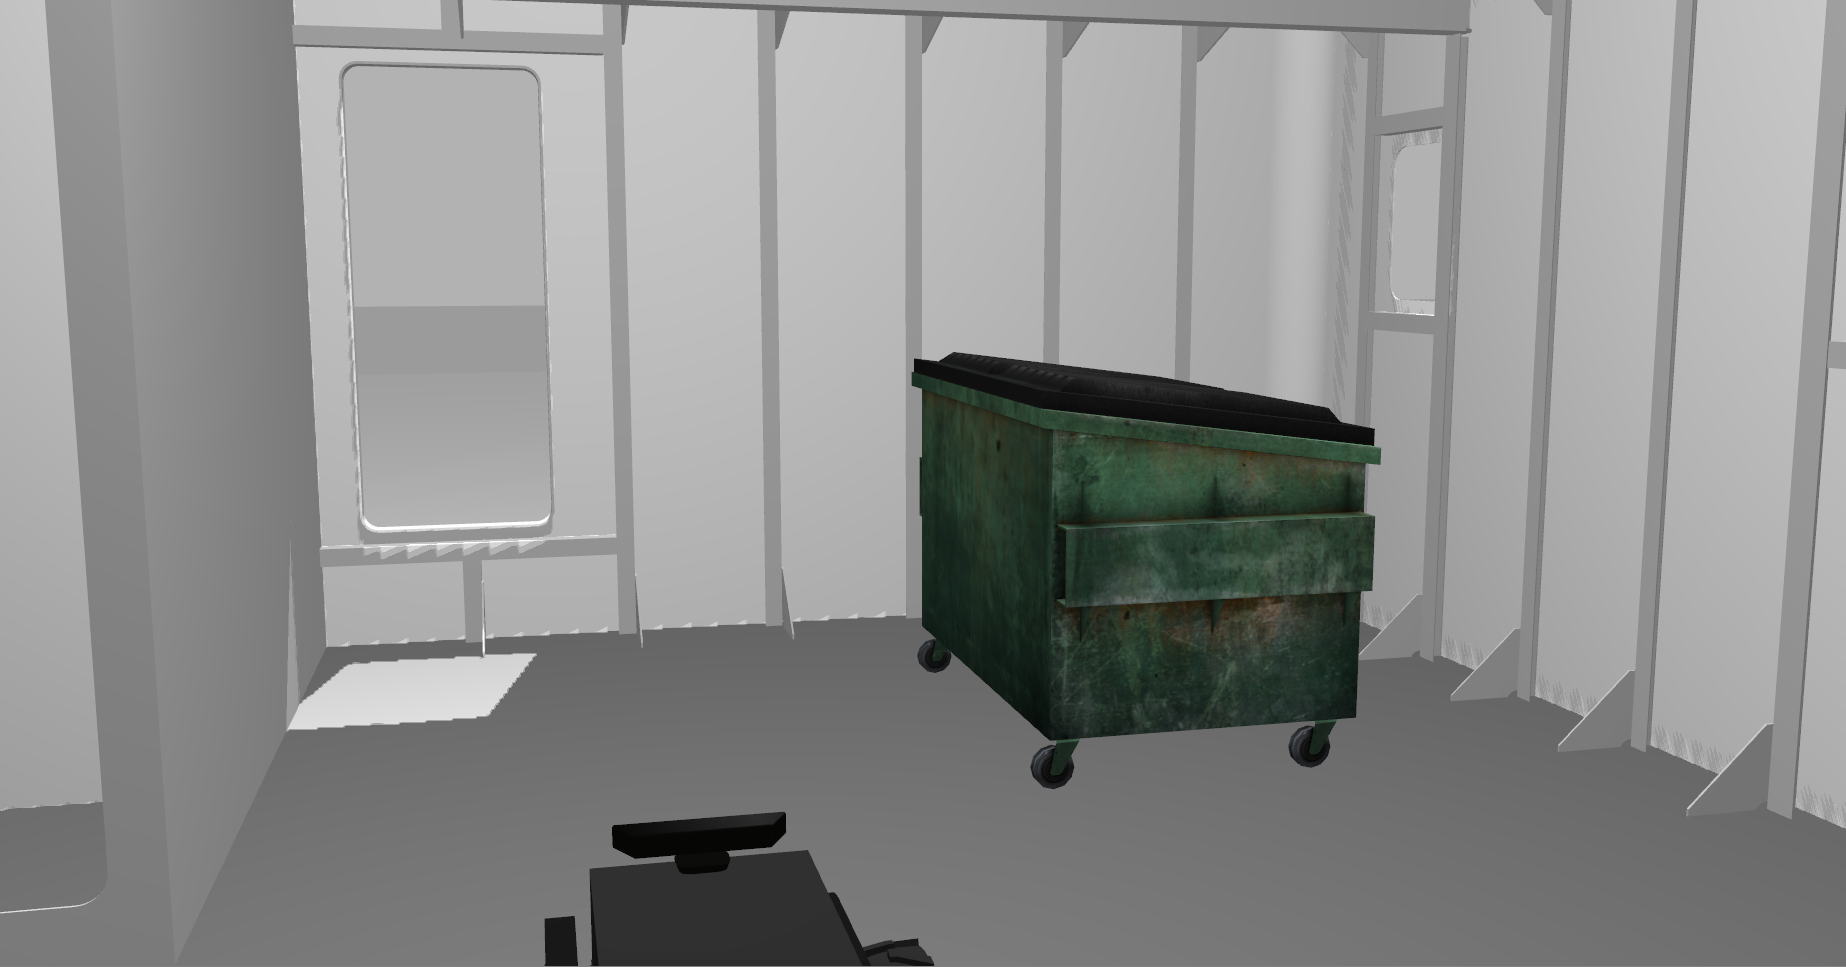
\includegraphics[width=\textwidth]{localization-system/outlier-detection-gazebo}
		\caption{Gazebo overview}
	\end{subfigure}
	\begin{subfigure}[ht]{0.35\textwidth}
		\centering
		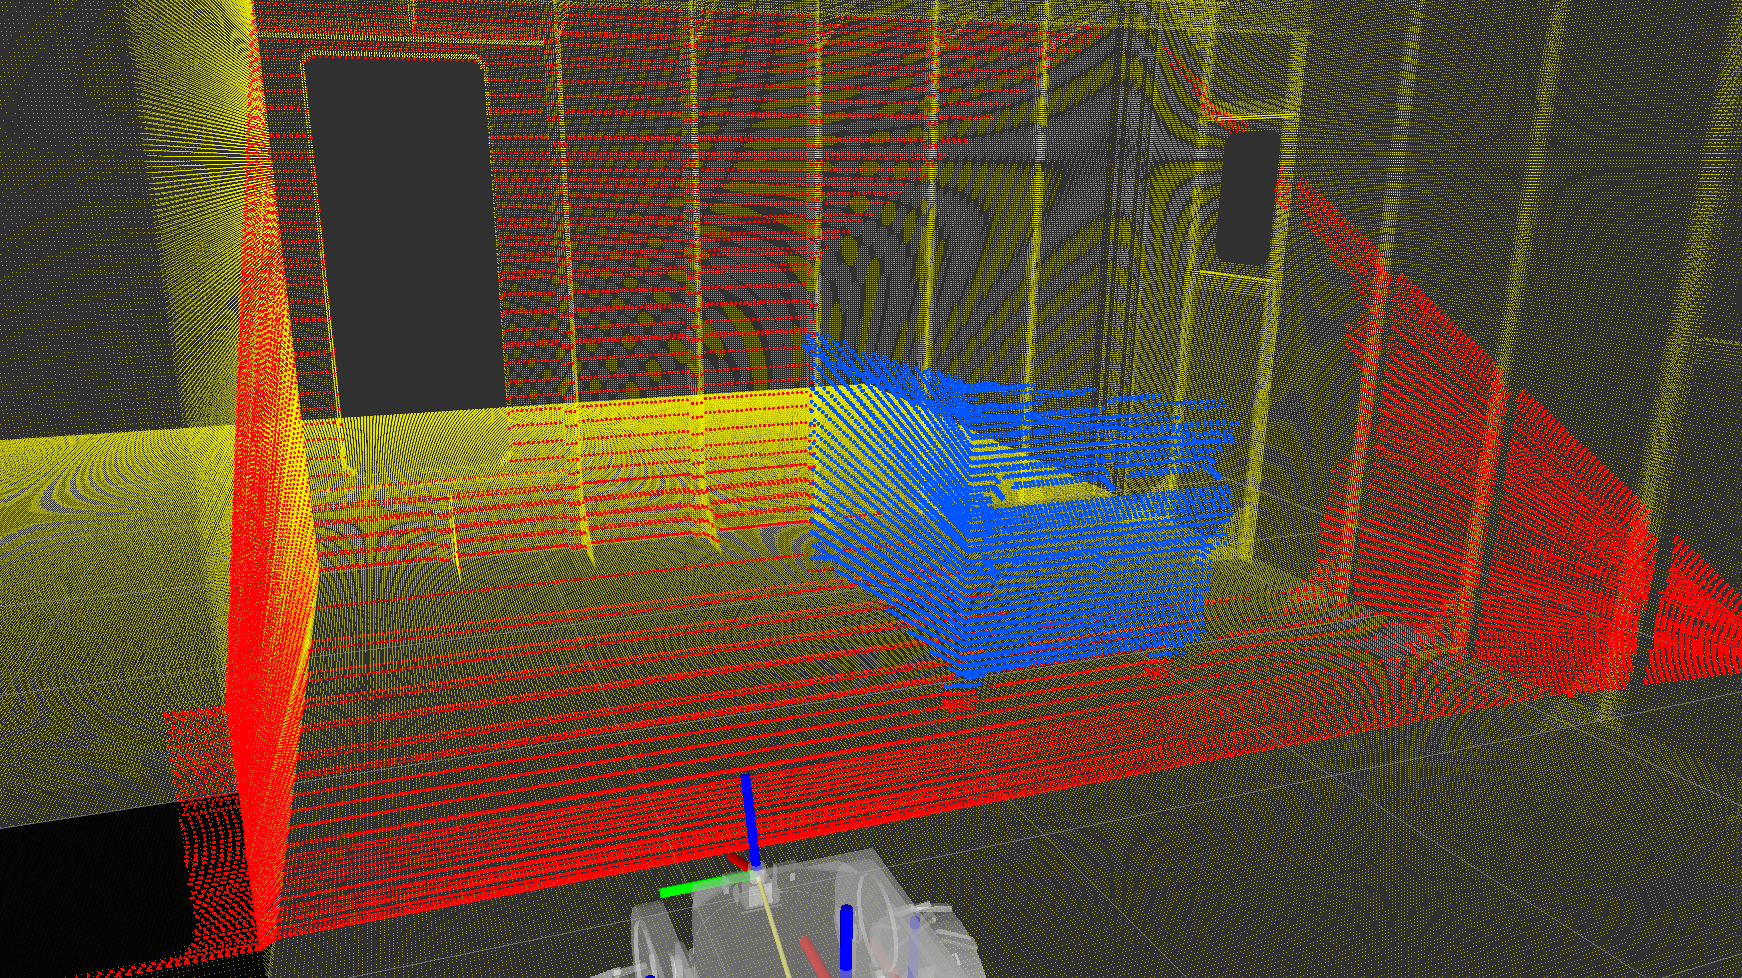
\includegraphics[width=\textwidth]{localization-system/outlier-detection}
		\caption{RViz overview}
	\end{subfigure}\hfill
	\caption{Point cloud registration with outlier detection}
	\label{fig:localization-system_outlier-detection}
\end{figure}


\subsection{Localization validation}

After a point cloud is registered by the localization system, several metrics are calculated in order to evaluate if a valid pose can be retrieved using the registration matrix.

The first computed metrics are the percentage of inliers and the \gls{rmse} of these inliers. If a minimum number of points was registered and the inlier percentage and root mean square error are acceptable (typical values for dynamic environments are at least 35\% of inliers with a \gls{rmse} lower than 30 mm), then the registration is considered successful. However, these registered points can be agglomerated in a small area and may not be representative of the robot location. As such, a second metric is computed that takes into account the angular distribution (drl::AngularDistributionAnalyzer) of these inliers. This metric gives a measurement of how reliable is this registration and is based on the fact that there is high confidence in a given pose estimation when there are correctly registered points all around the robot. The recommended parameters for this metric depend on the combined field of view of the sensors and if the robot is in an environment with geometry surrounding it. For typical use cases, a minimum of 60º of inliers angular distribution is reasonable.

The last metrics are the corrections that the registration matrix introduced. Given that the localization system will be in tracking mode most of the time, it is possible to define how far a new pose can be in relation to the previous accepted location and discard new poses that exceed a given threshold. This is useful to discard pose corrections that are very unlikely to happen, such as the robot moving half a meter between poses when it is expected to move only at 30 cm/s. These situations can happen when there is a sudden decrease in the field of view (that can occur due to sensor occlusion or malfunction) or when large unknown objects very similar to sections of the map appear into the field of view of the robot. For a typical robot moving slowly due to safety reasons, a maximum of 10 cm of translation and 10º of rotation between pose estimation might be reasonable (these thresholds depend on the sensors refresh rate and on the expected robot speed).

If all these metrics are within acceptable limits, then the robot pose can be computed by applying the matrix correction to the initial pose associated with the live sensor data.

If any of these metrics are not acceptable, then the system can be configured to simply discard this pose estimation and try to estimate the pose in the next sensor data updates or it can apply a tracking recovery attempt with a different registration algorithm (or the same algorithm with different parameters).

If several consecutive pose estimations are discarded (or a given time has passed since the last know pose), the system can have a second level of recovery that can be configured to use the initial pose estimation algorithms in order to finally estimate the global robot pose and reset the tracking state.


\subsection{Dynamic map update}

After performing a successful pose estimation, the \gls{drl} system can update the localization map by either integrating only the unknown objects or the full registered point cloud (it can also be used in conjunction with OctoMap \cite{Hornung2013} ir order to perform probabilistic map updates).

Integrating only the unknown objects is the recommended approach when there is a known map and the environment is expected to change gradually. This is also more efficient as only the points that need to be integrated are processed and ray traced in OctoMap. Moreover, integrating only new sections avoids map degradation or pollution (by sensor noise) of the detail of static areas (that were provided by \gls{cad} models).

On the other hand, integrating the full registered point cloud can be desirable if the map of the environment is very incomplete, very outdated or expected to change considerably during the operation of the robot.

Introducing new elements in the localization map may change slightly the reference coordinate system. As such, the \gls{drl} system in conjunction with OctoMap can use a static map for localization and continuously update the navigation map in order to keep valid previous localization / navigation waypoints and also allow better path planning for longer robot travels (given that some map sections might be obstructed by objects or new pathways might have become available).

